\documentclass[12pt,a4paper]{report}

\usepackage[ruled]{algorithm2e}
\usepackage{amsmath}
\usepackage{mathtools}
\usepackage{listings, xcolor}

\usepackage[italian]{babel}
\usepackage[T1]{fontenc}
\usepackage{geometry}
\usepackage{graphicx}
\usepackage{hyperref}
\usepackage[utf8]{inputenc}
\usepackage{subcaption}
\usepackage[nottoc,numbib]{tocbibind}
\usepackage{titlesec}
\usepackage{enumitem}

\usepackage{pgfplots}

\SetKwFor{While}{while}{}{end while}
\SetKwRepeat{Do}{do}{while}
\SetKwFor{For}{for}{}{end For}
\SetKwRepeat{Do}{do}{For}
\SetKw{KwGoTo}{go to}

\usepackage{courier}

\lstset{
	tabsize = 4,
	showstringspaces = false,
	commentstyle = \color{gray},
	keywordstyle = \color{blue},
	stringstyle = \color{red},
	rulecolor = \color{black},
	basicstyle = \small \ttfamily ,
	breaklines = true,
}

\newcommand*\justify{
  \fontdimen2\font=0.4em
  \fontdimen3\font=0.2em
  \fontdimen4\font=0.1em
  \fontdimen7\font=0.1em
  \hyphenchar\font=`\-
}

\titleformat{\chapter}[display]{\Huge\bfseries}{}{0pt}{\thechapter.\ }

\graphicspath{{figures/}}

% BEGIN DOCUMENT
\begin{document}

% BEGIN TITLE PAGE
\newgeometry{margin=1in}
\begin{titlepage}

	\centering
	
\includegraphics[width=0.34\textwidth]{logo-unipg}\par\vspace{1cm}
	\large{Tesina Finale di}\par
	\large{\textbf{Algoritmi e Strutture Dati}}\par
	\small{Corso di Laurea in Ingegneria Informatica ed Elettronica -- A.A. 2022-2023}\par
	\textsc{\small{Dipartimento di Ingegneria}}\par

	\vspace{0.5cm}
	docente\par
	Prof.~Emilio \textsc{DI GIACOMO}

	\vspace{2cm}
	\textbf{\huge{Calcolo dell'inviluppo convesso di un insieme di punti}}\par
	\vspace{0.2cm}
	  \textsc{Implementazione Algoritmo di Graham}\par
	
	\vspace{1.5cm}
	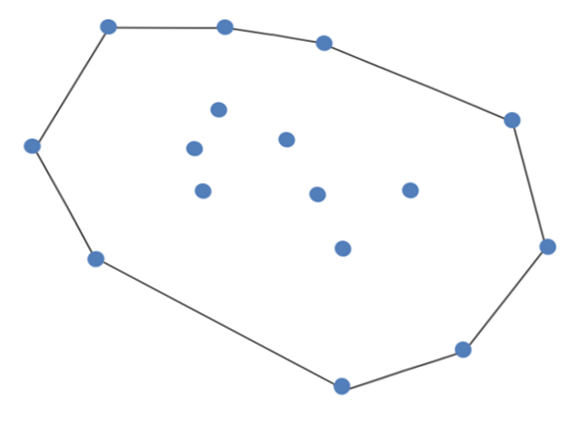
\includegraphics[width=0.6\textwidth]{CH.png}\par
 
	\vspace{1cm}
	\large{studenti}\par
	\vspace{0.5cm}
	\begin{tabular}{ l l l l }
	\large{330265} & \large{\textbf{Riccardo}} & \large{\textbf{Nicolini}} &        \large{riccardo.nicolini1@studenti.unipg.it}\\
	\large{329673} & \large{\textbf{Giovanni}} & \large{\textbf{Versiglioni}} &     \large{giovanni.versiglioni@studenti.unipg.it}\\
	\end{tabular}

    \vfill
    \raggedright
    \vspace{0.5cm}
    \small{\today}
\end{titlepage}
\restoregeometry
% END TITLE PAGE

\tableofcontents

\chapter{Descrizione del Problema}\label{ch:problema}
L'involucro (o inviluppo) convesso di un insieme di punti $Q$ ($CH(Q)$) è il più piccolo poligono convesso $P$ tale che ogni punto di $Q$ si trova sul perimetro di $P$ o nella sua parte interna.\\
Intuitivamente, pensando ogni punto di $Q$ come un chiodo che sporge da una tavola, l'involucro convesso è la forma che assumerebbe un elastico se circondasse tutti i chiodi.

\section{Applicazioni}
Nonostante la definizione del problema possa sembrare lontana dalla realtà, il problema del calcolo dell'inviluppo convesso di un insieme di punti trova riscontro in numerosi ambiti applicativi. Più in generale, la geometria computazionale (trattata nel seguito) è applicata a diversi campi dell'ingegneria e della matematica moderne, quali:\hspace{0.1cm}la grafica computerizzata, la robotica, la progettazione VLSI e CAD, la modellistica molecolare, la metallurgia, la statistica e molti altri.

\subsection*{\small{CONVEX RELAXATIONS}}
Una delle più interessanti applicazioni del problema è la possibilità di costruire rilassamenti convessi, cioè metodi per trovare il problema convesso più vicino a un problema non convesso che si vuole risolvere.

\subsection*{\small{EPIDEMIC TRACKING}}
Caratterizzare l'estensione spaziale di un'epidemia nella fase iniziale è molto importante per controllare l'evoluzione dell'epidemia. Ancora, questo può essere fatto calcolando l'involucro convesso che racchiude gli individui infetti in ogni istante di tempo.

\pagebreak

\subsection*{\small{COLLISION AVOIDANCE}}
L'inviluppo convesso di un insieme di punti è utile nella progettazione e nello sviluppo di sistemi di previsione delle collisioni in ambito robotico o automobilistico. Per comprendere al meglio come il problema proposto si possa presentare in questo caso d'uso, si considera l'esempio di un robot planare che vuole spostarsi da un punto A a un punto B. Il percorso più semplice e immediato da seguire è una linea retta che collega i punti A e B. Ora, potrebbero esserci degli ostacoli (punti nel piano) lungo tale percorso che impediscono al robot di raggiungere B. Se si vuole conoscere in tempo reale se il robot ha avuto una collisione con un ostacolo o se si vuole verificare che il percorso scelto sia privo di ostacoli, il modo più veloce di farlo è proprio quello di ricorrere all'involucro convesso. Infatti, l'involucro convesso è costruito attorno agli ostacoli e la posizione corrente del robot oppure i punti del percorso scelto sono testati verificando l'appartenenza alla parte interna dell'inviluppo convesso. Se ciascuno dei punti del percorso scelto si trova all'interno dell'involucro convesso, allora il robot incontrerà un ostacolo seguendo quel percorso e quindi si verificherà una collisione. Se, invece, tutti i punti del percorso sono all'esterno dell'involucro convesso, allora il percorso è privo di ostacoli e il robot non andrà a collidere con alcun ostacolo andando verso B.

\begin{figure}[ht]
    \centering
    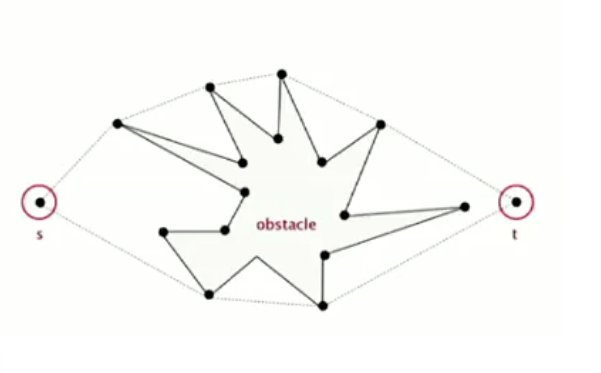
\includegraphics[width=0.75\linewidth]{collisionAvoidance.png}
    \caption{Involucro convesso e previsione delle collisioni.}
\end{figure}

\pagebreak

\section{Geometria Computazionale}
La geometria computazionale è la branca dell'informatica che studia gli algoritmi per risolvere i problemi geometrici.

\subsection*{\small{PRODOTTO VETTORIALE}}
Considerati i vettori $p_1$ e $p_2$, il prodotto vettoriale $p_1 \times p_2$ può essere interpretato come l'area con segno del parallelogramma formato dai punti $(0, 0), p_1, p_2, p_1 + p_2 = (x_1 + x_2, y_1 + y_2)$.\\
Equivalentemente, si può interpretare il prodotto vettoriale come il determinante di una matrice:
\[
p_1 \times p_2 = \det\begin{pmatrix}
                    x_1 & x_2\\ 
                    y_1 & y_2 
                    \end{pmatrix}
= x_1y_2 - x_2y_1
\]\\
Se il prodotto vettoriale $p_1 \times p_2$ è:
\begin{itemize}
    \item[-] positivo, allora $p_1$ segue in senso orario $p_2$ nella rotazione attorno all'origine;
    \item[-] negativo, allora $p_1$ segue in senso antiorario $p_2$ nella rotazione attorno all'origine;
    \item[-] nullo, allora i vettori sono collineari, in quanto puntano nella stessa direzione o in direzioni opposte.
\end{itemize}

\begin{figure}[ht]
\centering
 \begin{subfigure}{.4\textwidth}
    \centering
    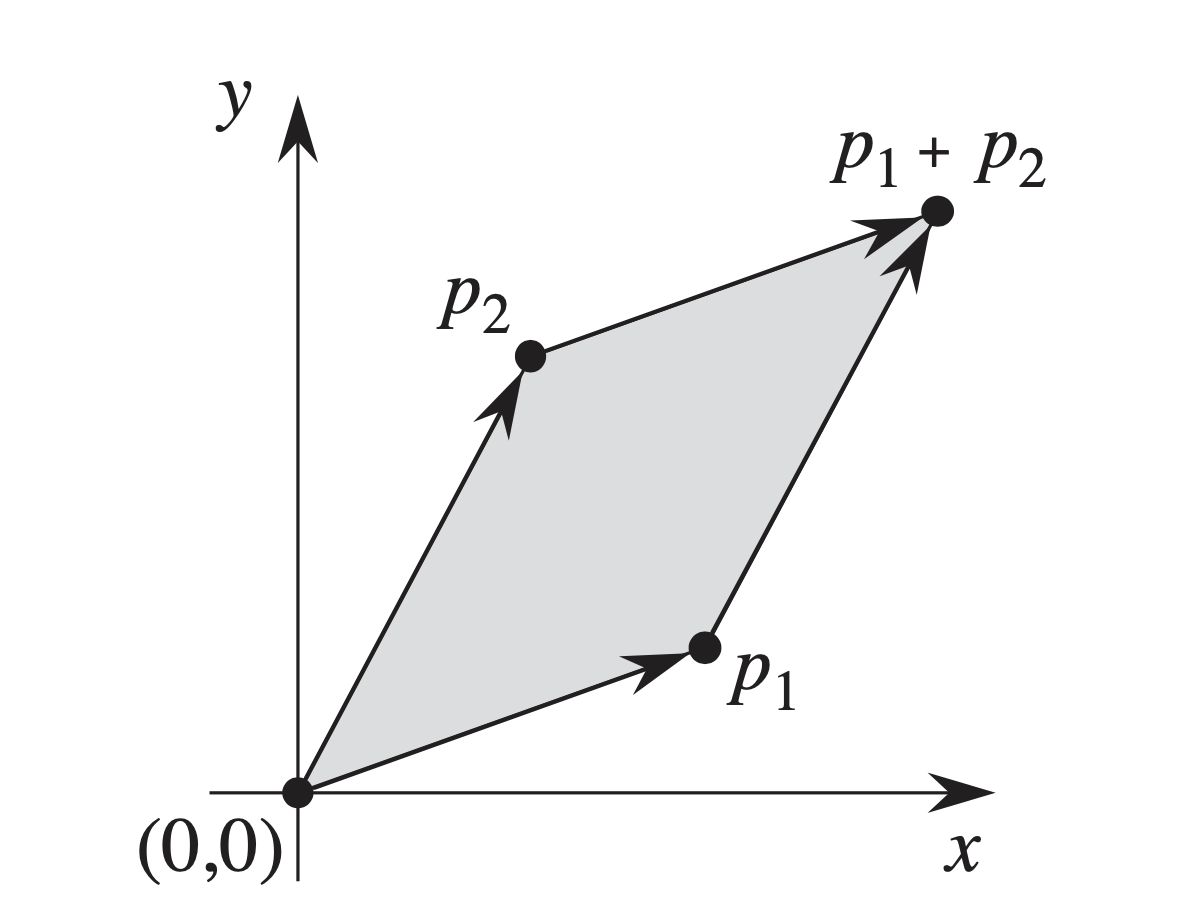
\includegraphics[width=1\linewidth]{crossproduct.png}
    \caption{}
    \label{fig:crossproduct}
 \end{subfigure}
 \begin{subfigure}{.4\textwidth}
    \centering
    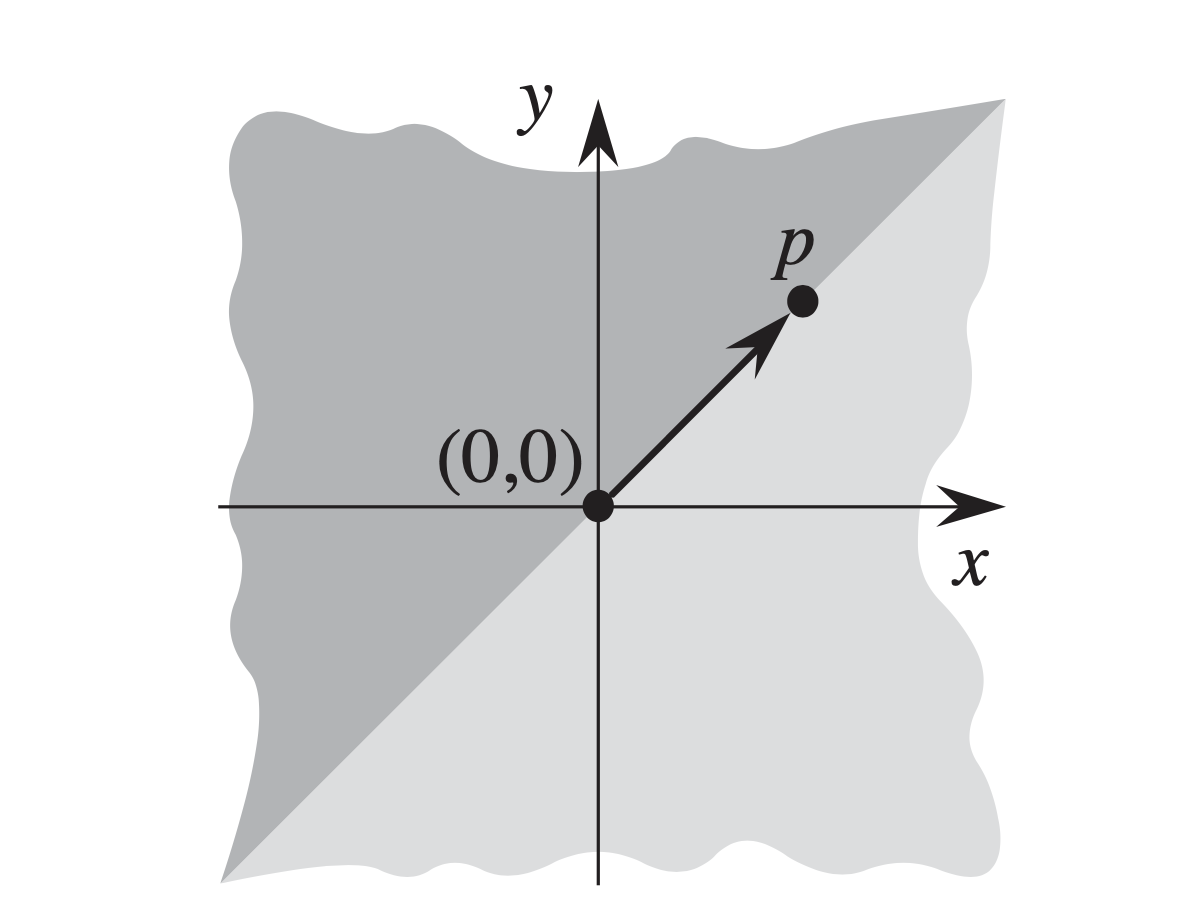
\includegraphics[width=1\linewidth]{crossproductturn.png}
    \caption{}
    \label{fig:crossproductturn}
 \end{subfigure}
 \caption{\textbf{\ref{fig:crossproduct}} Il prodotto vettoriale dei vettori $p_1$ e $p_2$ è l'area con segno del parallelogramma indicato. \textbf{\ref{fig:crossproductturn}} La zona di colore grigio chiaro contiene i vettori che seguono in senso orario il vettore $p$, quella di colore grigio scuro contiene i vettori che seguono in senso antiorario il vettore $p$.}
\end{figure}

Poter determinare, tramite il prodotto vettoriale definito, il senso di rotazione di un segmento nei confronti di un altro (applicato nello stesso punto), gioca un ruolo fondamentale all'interno della geometria computazionale.\\
Per determinare se un vettore $\overrightarrow{p_0p_1}$ segue in senso orario il vettore $\overrightarrow{p_0p_2}$ attorno all'estremo $p_0$, si effettua prima di tutto una traslazione ponendo $p_0$ come origine.\\
Si ottengono quindi i seguenti due nuovi vettori: 
\[ {p_1}' = ((x_1 - x_0),(y_1 - y_0))
\hspace{1cm}
{p_2}' = ((x_2 - x_0),(y_2 - y_0)) \]\\
Calcolando il prodotto vettoriale si ottiene:
\[{p_1}' \times {p_2}' = (p_1 - p_0) \times (p_2 - p_0) = (x_1 - x_0)(y_2 - y_0) - (x_2 - x_0)(y_1 - y_0)\]\\
Se il prodotto vettoriale ${p_1}' \times {p_2}'$ è:
\begin{itemize}
    \item[-] positivo, allora $\overrightarrow{p_0p_1}$ segue in senso orario $\overrightarrow{p_0p_2}$;
    \item[-] negativo, allora $\overrightarrow{p_0p_1}$ segue in senso antiorario $\overrightarrow{p_0p_2}$.
\end{itemize}

\pagebreak

\subsection*{\small{SVOLTA DI DUE SEGMENTI CONSECUTIVI}}
Analizzato il caso in cui i due segmenti hanno la stessa origine, si vuole determinare se due segmenti consecutivi $\overline{p_0p_1}$ e $\overline{p_1p_2}$ svoltano a destra o a sinistra nel punto $p_1$. Occorre quindi determinare in che senso ruota l'angolo $\angle p_0p_1p_2$.\\
Il prodotto vettoriale definito consente di rispondere a quest'ultima domanda senza dover calcolare l'angolo, verificando se il vettore $\overrightarrow{p_0p_2}$ è ruotato in senso orario o antiorario rispetto al vettore $\overrightarrow{p_0p_1}$.\\
Si calcola quindi il prodotto vettoriale $(p_2 - p_0) \times (p_1 - p_0)$ e se il segno è:
\begin{itemize}
    \item[-] positivo, indica una rotazione in senso orario, cioè una svolta a destra in $p_1$ (Figura \textbf{\ref{fig:clockwise}});
    \item[-] negativo, indica una rotazione in senso antiorario, cioè una svolta a sinistra in $p_1$ (Figura \textbf{\ref{fig:anticlockwise}});
    \item[-] nullo, significa che i tre punti sono collineari. 
\end{itemize}

\begin{figure}[ht]
\centering
 \begin{subfigure}{.4\textwidth}
    \centering
    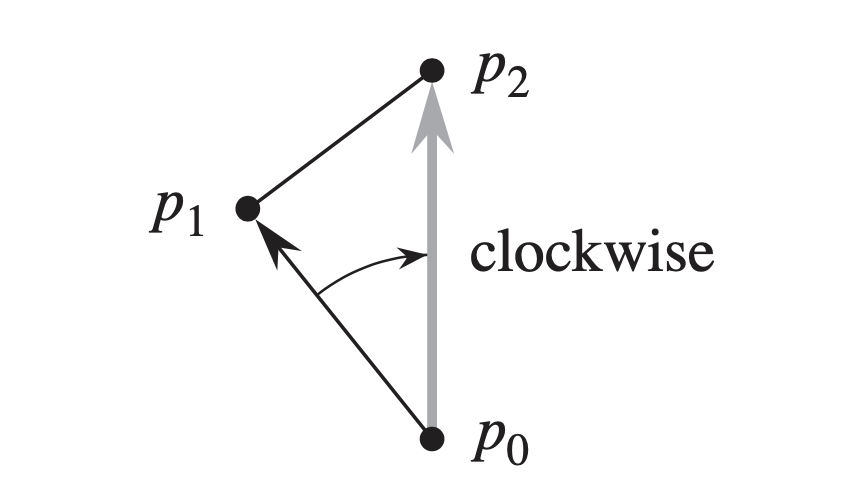
\includegraphics[width=1\linewidth]{clockwise.png}
    \caption{Rotazione in senso orario.}
    \label{fig:clockwise}
 \end{subfigure}
 \begin{subfigure}{.4\textwidth}
    \centering
    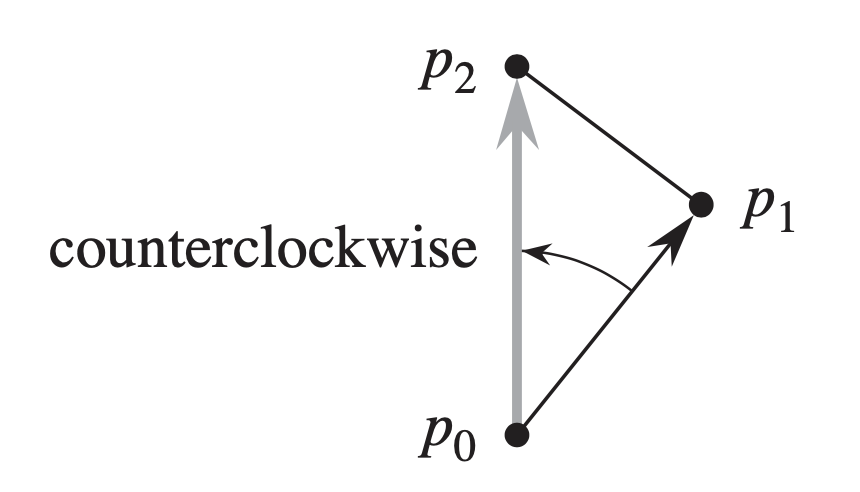
\includegraphics[width=1\linewidth]{anticlockwise.png}
    \caption{Rotazione in senso antiorario.}
    \label{fig:anticlockwise}
 \end{subfigure}
 \caption{Svolta di due segmenti consecutivi.}
\end{figure}

\section{Metodi di Calcolo}
Esistono diversi algoritmi che risolvono il problema del calcolo dell'inviluppo convesso di un insieme di punti. Prima di parlare dell'algoritmo di Graham, oggetto di studio della tesina, è importante conoscere altri metodi di calcolo per avere un'idea generale sul tempo di esecuzione, quindi poter trarre conclusioni sull'efficacia.\\

\subsection*{\small{METODO INCREMENTALE}}
Questo metodo ordina i punti da sinistra a destra, producendo una sequenza $\langle p_1, ..., p_n\rangle$. All'i-esimo stadio, l'involucro convesso $CH(\{p_1, ..., p_{i-1}\})$ degli $i - 1$ punti più a sinistra viene aggiornato in base all'i-esimo punto da sinistra, formando così $CH(\{p_1, ..., p_i\})$. Il metodo può essere implementato in modo da richiedere un tempo pari a $O(n\hspace{0.05cm}lgn)$.

\subsection*{\small{METODO DIVIDE ET IMPERA}}
Questo metodo divide in un tempo $\Theta(n)$ l'insieme di $n$ punti in due sottoinsiemi, uno contenente gli  $\lceil n/2 \rceil$ punti più a sinistra e l'altro contenente gli $\lfloor n/2 \rfloor$ punti più a destra. L'involucro convesso dei sottoinsiemi è calcolato in modo ricorsivo e le soluzioni sono combinate in un tempo $O(n)$.
Il tempo di esecuzione è quindi $T(n) = 2T(n/2) + O(n) \Rightarrow O(n\hspace{0.05cm}lgn)$.

\subsection*{\small{METODO PRUNE AND SEARCH}}
Questo metodo trova la porzione superiore (catena superiore) dell'involucro convesso eliminando ripetutamente una frazione dei punti restanti, ottenendo così la catena superiore dell'involucro convesso. Ripete poi lo stesso procedimento per la catena inferiore. È asintoticamente il più veloce, infatti se $CH$ contiene $h$ vertici viene eseguito in un tempo $O(n\hspace{0.05cm}lg\hspace{0.01cm}h)$.

\subsection*{\small{ALGORITMO DI JARVIS}}
L'algoritmo di Jarvis calcola l'involucro convesso di un insieme di punti $Q$ adottando una tecnica di "impacchettamento" o "confezionamento" dei regali ("gift wrapping"). A differenza dell'algoritmo di Graham, trattato nel seguito, questo algoritmo consente di calcolare l'involucro convesso di un insieme di punti non necessariamente planari, ma anche a dimensioni maggiori o uguali a tre. Il problema dell'involucro convesso formulato per dimensioni maggiori di due è analogo, ma:
\begin{itemize}
    \item[-] in uno spazio tridimensionale diventa il più piccolo poliedro convesso tale che ogni punto dell'insieme di input si trova al suo interno o sulla sua superficie esterna;
    \item[-] in uno spazio n-dimensionale diventa il più piccolo politopo convesso tale che ogni punto dell'insieme di input si trova al suo interno o sulla frontiera.
\end{itemize}
Intuitivamente, l'idea di fondo dell'algoritmo è quella di simulare l'operazione di impacchettare con un foglio di carta l'insieme $Q$ dei punti dati. Si parte ancorando l'estremità del foglio di carta al punto più basso dell'insieme (punto di partenza scelto esattamente come in Graham). Questo punto è sicuramente un vertice dell'involucro convesso. Ora, si tira la carta verso destra (ad esempio) per tenderla e poi la si tira verso l'alto fin quando non si tocca un punto di $Q$. Mantenendo tesa la carta, si continua ad impacchettare l'insieme dei vertici fino a che non si ritorna al punto scelto in partenza, completando il desiderato involucro convesso.\\

Questo algoritmo viene eseguito in tempo $O(nh)$, dove $h$ è il numero di vertici di $CH(Q)$. Quando $h$ è $O(lgn)$, l'algoritmo di Jarvis è asintoticamente più veloce dell'algoritmo di Graham, che richiede sempre $O(n\hspace{0.05cm}lgn)$ per essere eseguito (indipendentemente dal numero di vertici dell'involucro convesso che si ottiene).

\chapter{Algoritmi e Strutture Dati Implementati}\label{ch:implementazione}
Nel seguito si presenta una possibile soluzione al problema dell'involucro convesso: l'algoritmo di Graham.

\section{Descrizione delle Strutture Dati}
L'algoritmo di Graham risolve il problema dell'involucro convesso, mantenendo i punti candidati in una pila $P$. Ogni punto dell'insieme di input $Q$ viene inserito una sola volta nella pila: se non fa parte di $CH(Q)$ viene rimosso dalla pila, altrimenti è mantenuto.
Alla fine dell'esecuzione la pila $P$ contiene esattamente i vertici di $CH(Q)$ in ordine antiorario.\\
L'algoritmo deve poter accedere all'elemento affiorante della pila e al precedente, e deve inoltre poter aggiungere e rimuovere elementi dalla pila, pertanto si implementano le seguenti operazioni:

\vspace{0.5cm}

\noindent \texttt{TOP(P)\\
return P.A[P.top]}

\vspace{0.4cm}

\noindent \texttt{NEXT-TO-TOP(P)\\
return P.A[P.top - 1]}

\vspace{0.4cm}

\noindent \texttt{PUSH(P,x)\\
P.top = P.top + 1\\
P.A[P.top] = x}

\vspace{0.4cm}

\noindent \texttt{POP(P)\\
P.top = P.top - 1\\
return P.A[P.top + 1]}

\section{Descrizione dell'Algoritmo}
Nella fase iniziale l'algoritmo seleziona il punto $p_0$ con coordinata y minima. Se più punti si trovano sulla stessa ordinata, si sceglie (tra questi) il punto con coordinata x minima. Dato che non esiste punto in $Q$ sotto $p_0$ ed eventualmente i punti che si trovano sulla sua stessa ordinata sono alla sua destra, $p_0$ è un vertice di $CH(Q)$.

\vspace{0.5cm}

Si procede ordinando i restanti punti di $Q$ in funzione degli angoli polari rispetto a $p_0$, mediante il metodo dei prodotti vettoriali. Se ci sono più punti con lo stesso angolo polare rispetto a $p_0$ si mantiene solo quello più lontano. I punti individuati sono inseriti nell'array $\langle p_1, p_2, ..., p_m \rangle$. Poiché i punti sono ordinati in funzione degli angoli polari, essi risultano ordinati in senso antiorario rispetto a $p_0$.\\
I punti $p_1$ e $p_m$ sono vertici di $CH(Q)$ perché sono rispettivamente i punti con angolo polare minore e maggiore in riferimento a $p_0$.

\vspace{0.5cm}

Si crea quindi una pila $P$ (inizialmente vuota) nella quale si inseriscono i punti $p_0, p_1, p_2$.

\vspace{0.5cm}

Ad ogni iterazione del ciclo for, cioè per ogni punto $p_i, i = 3, ..., m$, un ciclo while valuta in che senso ruota l'angolo formato dai punti $\angle (\texttt{NEXT-TO-TOP(P)}, \texttt{TOP(P)}, p_i)$.

Se l'angolo:
\begin{itemize}
    \item[-] ruota verso destra (prodotto vettoriale positivo), viene rimosso l'elemento affiorante della pila $P$, in quanto non appartiene all'involucro di convesso dei punti $\langle p_0, ..., p_i \rangle$;
    \item[-] ruota verso sinistra (prodotto vettoriale negativo), l'elemento affiorante non viene rimosso dalla pila $P$, in quanto appartiene all'involucro di convesso dei punti $\langle p_0, ..., p_i \rangle$;
    \item[-] non ruota (prodotto vettoriale nullo), viene rimosso l'elemento affiorante della pila $P$, in quanto nessun vertice di un poligono convesso può essere una combinazione convessa di altri vertici del poligono (cioè, non possono esistere tre vertici dell'involucro convesso colllineari, per definizione di involucro convesso).
\end{itemize}

Si va avanti fino a che il ciclo for non termina la scansione di tutti i punti di $\langle p_1, p_2, ..., p_m \rangle$, visitando l'ultimo punto $p_m$.\\
Infine, l'algoritmo restituisce la pila $P$ contenente i vertici dell'involucro convesso ordinati in senso antiorario rispetto a $p_0$.

\pagebreak

Di seguito lo pseudocodice dell'algoritmo di Graham.

% BEGIN GRAHAM ALGORITHM
\begin{algorithm}[ht]
\caption{GRAHAM-SCAN(Q)}\label{alg:graham}

\vspace{0.3cm}

\nl Sia $p_0$ il punto di $Q$ con la coordinata $y$ minima o il punto più a sinistra se più più punti hanno la stessa $y$ minima

\vspace{0.3cm}

\nl Siano $\langle p_1, p_2, ..., p_m \rangle$ i restanti punti di $Q$ ordinati rispetto agli angoli polari in senso antiorario intorno a $p_0$ (avendo rimosso tutti i punti che hanno lo stesso angolo, tranne quello che è più lontano da $p_0$)

\vspace{0.3cm}

\nl Sia $P$ una pila vuota

\vspace{0.3cm}

\nl $PUSH(p_0, P)$

\vspace{0.1cm}

\nl $PUSH(p_1, P)$

\vspace{0.1cm}

\nl $PUSH(p_2, P)$

\vspace{0.3cm}

\nl \For{$i=3$ \KwTo $m$} {
\vspace{0.1cm}
\nl \While{$\angle (\texttt{NEXT-TO-TOP(P)}, \texttt{TOP(P)}, p_i)$ svolta non a sinistra} {
\vspace{0.1cm}
\nl $POP(P)$
}
\vspace{0.1cm}
\nl $PUSH(P_i,P)$
}
\vspace{0.3cm}
\nl \Return P
\end{algorithm}
% END GRAHAM ALGORITHM

\begin{figure}[ht]
    \centering
    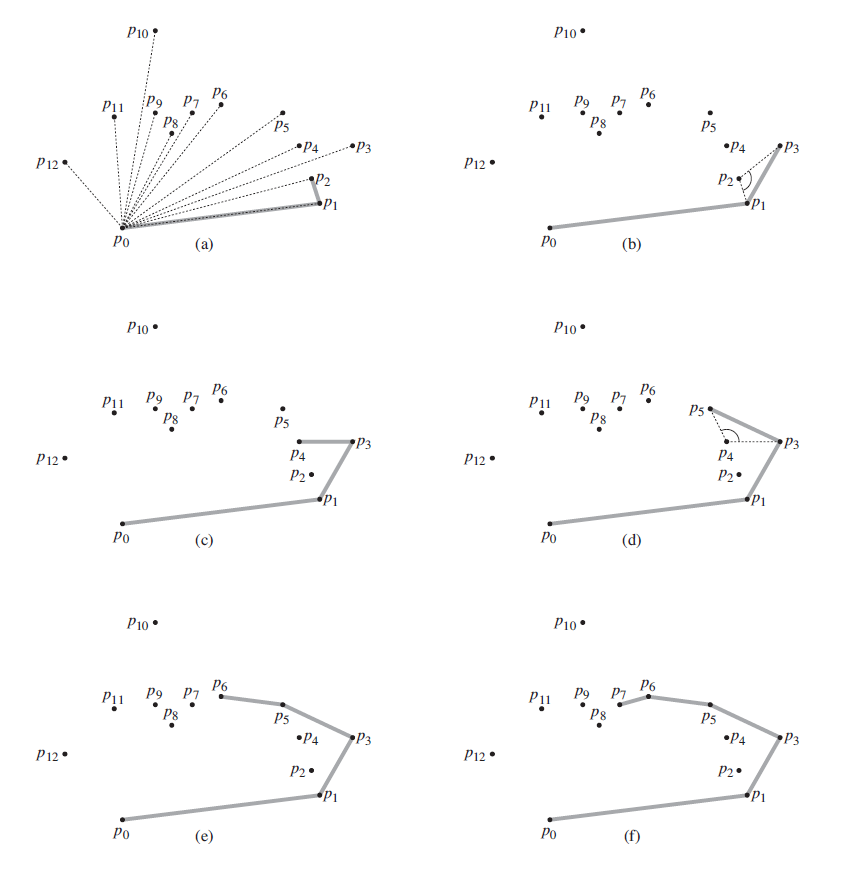
\includegraphics[width=1\linewidth]{ImmaginiGraham.png}
    \caption{Esempio di esecuzione di \texttt{GRAHAM-SCAN(Q)}.}
    \label{fig:immGraham1}
\end{figure}

\pagebreak

\begin{figure}[ht]
    \centering
    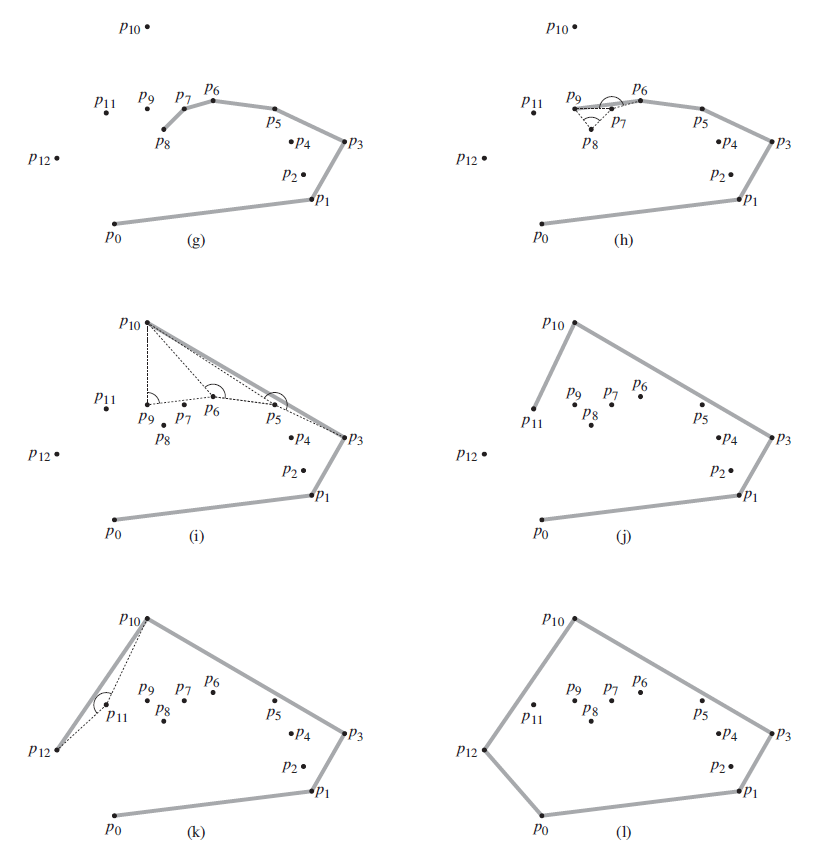
\includegraphics[width=1\linewidth]{ImmaginiGraham2.png}
    \caption{Esempio di esecuzione di \texttt{GRAHAM-SCAN(Q)}.}
    \label{fig:immGraham2}
\end{figure}

\chapter{Analisi}\label{ch:anallisi}

\section{Analisi della Correttezza}\label{ch:correttezza}
Si vuole dimostrare che l'esecuzione dell'algoritmo di Graham su un insieme di punti $Q$, con $|Q| \geq 3$, fornisca in output una pila $P$ contenente, dal basso verso l'alto, esattamente i vertici dell'involucro convesso di $Q$ in ordine antiorario.

\vspace{0.5cm}

\noindent Sia $Q_i = \{ p_0, p_1, ..., p_i \}, i = 2, 3, ..., m$.\\
I punti in $Q - Q_m$ sono quelli che sono stati rimossi (alla riga 2) perché avevano lo stesso angolo polare rispetto a $p_0$ di qualche punto in $Q_m$, ma erano meno distanti da $p_0$ rispetto al punto con cui condividevano l'angolo polare.\\
Questi punti non fanno parte dell'involucro convesso di $Q$, quindi è equivalente calcolare l'involucro convesso di $Q$ o $Q_m$:
\[  CH(Q) = CH(Q_m) \]\\
Quindi, basta dimostrare che l'esecuzione dell'algoritmo di Graham sull'insieme $Q_m$ fornisca in output uno stack $S$ contenente, dal basso verso l'alto, esattamente i vertici dell'involucro convesso di $Q_m$ in ordine antiorario.

\subsection*{\small{INVARIANTE DI CICLO}}
All'inizio di ogni iterazione del ciclo for (righe 7-10), la pila $P$ contiene, dal basso verso l'alto, esattamente i vertici di $CH(Q_{i-1})$ in ordine antiorario.

\vspace{0.5cm}

\noindent \textbf{Inizializzazione.}\\
L'invariante è vera prima della prima iterazione del ciclo for, perché in quel momento la pila $P$ contiene esattamente i vertici di $Q_2$. Questi tre vertici formano il proprio involucro convesso e sono memorizzati nella pila in ordine antiorario, dal basso verso l'alto.

\pagebreak

\noindent \textbf{Conservazione.}\\
\textit{Passo 1.}\\
Prima di ogni iterazione del ciclo for l'elemento affiorante di $P$ è il punto $p_{i-1}$, che era stato inserito nella pila alla fine della precedente iterazione.\\
Sia $p_j$ il punto in cima alla pila dopo l'esecuzione del ciclo while, ma prima che la riga 10 inserisca il punto $p_i$.\\
Sia $p_k$ il punto appena sotto $p_j$ nella pila.\\
Quando $p_j$ è il punto in cima alla pila e non è stato ancora inserito $p_i$, la pila contiene esattamente gli stessi punti che conteneva dopo l'iterazione $j$ del ciclo for.\\
Quindi, per l'invariante di ciclo, in quel momento $P$ contiene esattamente i vertici di $CH(Q_j)$, che appaiono in ordine antiorario, dal basso verso l'alto.

\vspace{0.3cm}


\noindent Mantenendo l'ipotesi che $p_i$ (durante l'iterazione $i$ corrente) non è ancora stato inserito nella pila e tenendo conto che:
\begin{itemize}
    \item[-] l'angolo polare di $p_i$ rispetto a $p_0$ è maggiore di quello di $p_j$;
    \item[-] l'angolo $\angle p_kp_jp_i$ effettua una svolta a sinistra (altrimenti $p_j$ sarebbe stato rimosso);
\end{itemize}
si nota che, poiché la pila contiene esattamente i vertici di $CH(Q_j)$, una volta inserito $p_i$, la pila conterrà esattamente i vertici di $CH(Q_j \cup \{p_i\})$, ancora in ordine antiorario, dal basso verso l'alto.

\begin{figure}[ht]
    \centering
    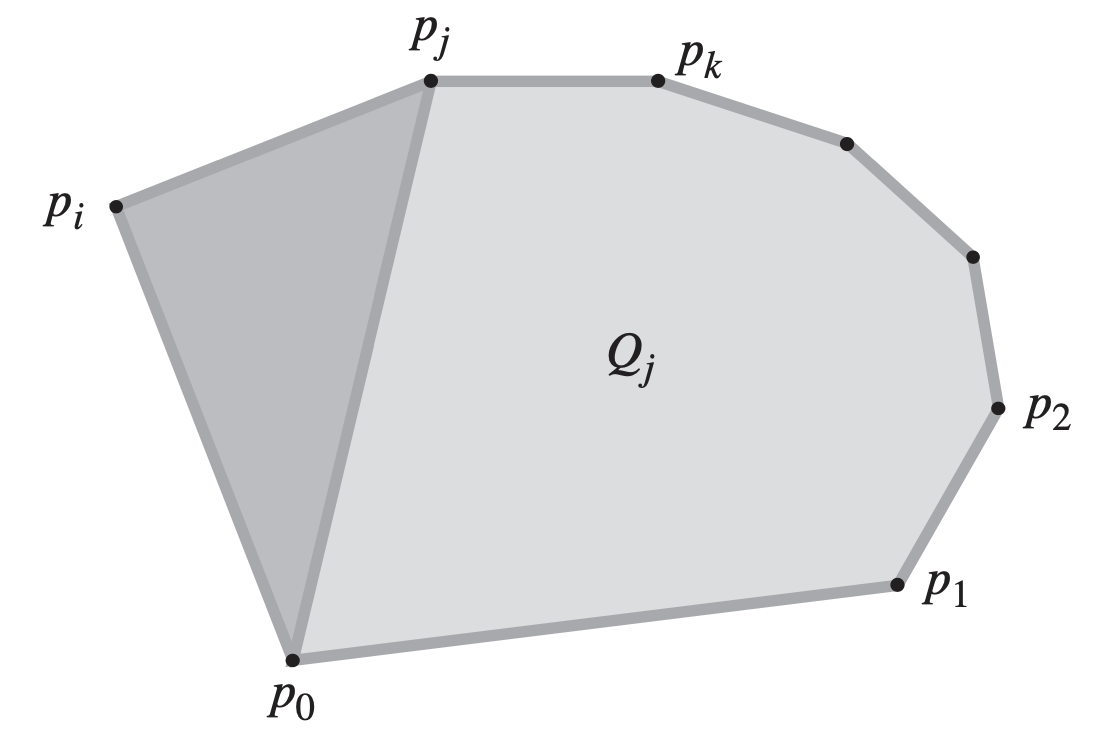
\includegraphics[width=0.55\linewidth]{dimStep1.png}
    \caption{Passo 1.}
    \label{fig:dimStep1}
\end{figure}

\pagebreak

\noindent \textit{Passo 2.}\\
Nel seguito si dimostra che:
\[ CH(Q_j \cup \{p_i\}) = CH(Q_i)\]\\
Sia $p_t$ un generico punto che è stato rimosso durante l'iterazione $i$ del ciclo for.\\
Sia $p_r$ il punto appena sotto $p_t$ nella pila nel momento in cui $p_t$ viene rimosso.\\
Si ottiene che:
\begin{itemize}
    \item[-] l'angolo polare di $p_t$ rispetto a $p_0$ è maggiore di quello di $p_r$;
    \item[-] l'angolo $\angle p_rp_tp_i$ effettua una svolta non a sinistra.
\end{itemize}
In altre parole, $p_t$ deve trovarsi o nella parte interna o su un lato del triangolo formato da $p_0, p_r, p_i$, ma non sui vertici di quest ultimo.\\
Dato che $p_t$ è all'interno di un triangolo formato da tre punti di $Q_i$, non può essere un vertice dell'involucro convesso di $Q_i$; quindi:
\[ CH(Q_i - \{p_t\}) = CH(Q_i) \]

\begin{figure}[ht]
    \centering
    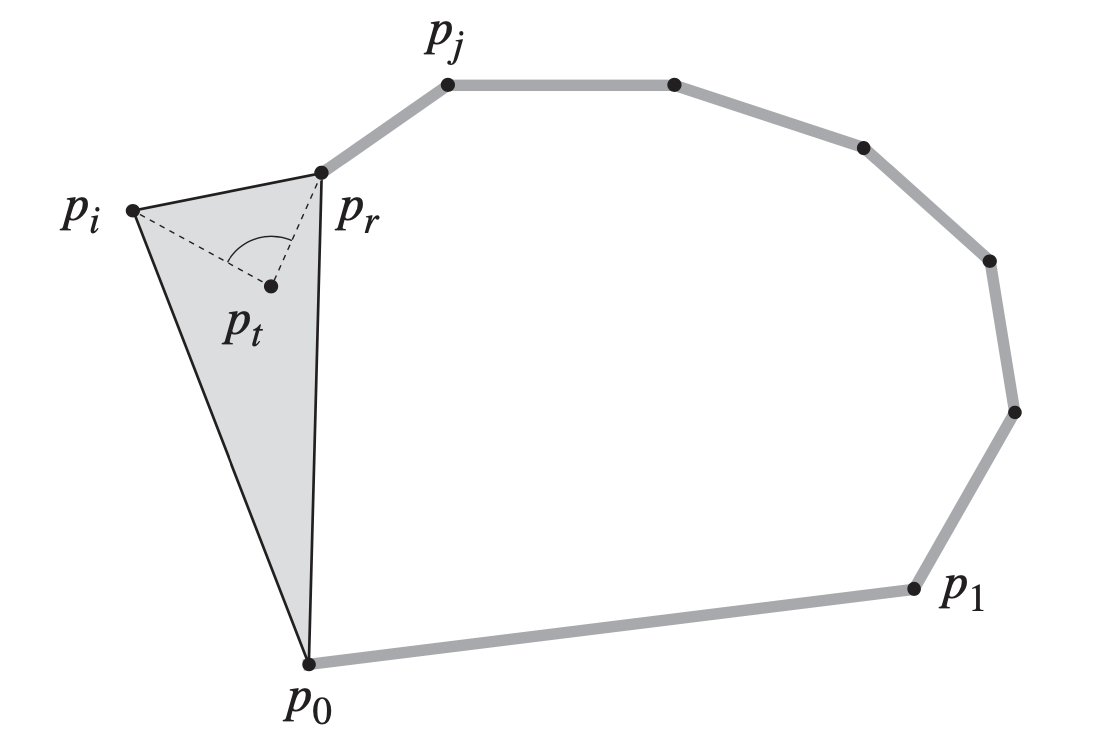
\includegraphics[width=0.55\linewidth]{dimStep2.png}
    \caption{Passo 2.}
    \label{fig:dimStep2}
\end{figure}

\noindent Sia $P_i$ l'insieme dei punti che sono stati rimossi durante l'iterazione $i$ del ciclo for.\\
Dato che l'uguaglianza dimostrata al \textit{Passo 2} è valida per ogni punto di $P_i$, la si può applicare ripetutamente per dimostrare che:
\[ CH(Q_i - P_i) = CH(Q_i) \]\\
Ma $Q_i - P_i = Q_j \cup \{p_i\}$, quindi:
\[ CH(Q_i - P_i) = CH(Q_j \cup \{p_i\}) = CH(Q_i) \]\\

\vspace{0.3cm}

\noindent In conclusione, per ogni iterazione $i$, una volta inserito $p_i$, la pila $P$ contiene esattamente i vertici di $CH(Q_i)$ in ordine antiorario, dal basso verso l'alto.

\vspace{0.5cm}

\noindent \textbf{Conclusione.}\\
Quando il ciclo termina ($i = m + 1$) l'invariante di ciclo implica che la pila contiene, dal basso verso l'alto, esattamente i vertici, in ordine antiorario, di $CH(Q_M) = CH(Q)$. 

\section{Analisi della Complessità}\label{ch:complessita}
\noindent Si dimostra nel seguito che il tempo di esecuzione di \texttt{GRAHAM-SCAN(Q)} è $O(nlgn)$, con $n = |Q|$.\\
L'ordinamento dei punti secondo l'angolo polare (riga 2) richiede un tempo $O(nlgn)$, se si usa merge sort o heapsort. La rimozione di tutti i punti che hanno lo stesso angolo polare, tranne il punto più lontano, richiede un tempo $O(n)$ (scansione lineare).\\
Le righe 3-6 richiedono un tempo costante, in quanto il loro tempo di esecuzione non dipende dalla dimensione dell'input.\\
Dato che $m \leq n - 1$, il ciclo for (righe 7-10) viene eseguito al più $n - 3$ volte. Escludendo il ciclo while annidato, nel corpo del ciclo for è presente (ad ogni iterazione) una \texttt{PUSH()}, che richiede un tempo di esecuzione costante ($O(1)$). Pertanto, escludendo il ciclo while, il ciclo for richiede complessivamente un tempo lineare ($O(n)$).\\
Utilizzando il metodo dell'aggregazione, si dimostra che il ciclo while richiede complessivamente un tempo $O(n)$. Per $i = 0, ..., m$, ogni punto $p_i$ viene inserito nella pila $P$ una sola volta. Inoltre, si nota che c'è al più un'operazione \texttt{POP()} per ogni operazione \texttt{PUSH()}, infatti ad ogni iterazione viene esguita una \texttt{PUSH()}, ma all'iterazione successiva la \texttt{POP()} può essere chiamata oppure no, a seconda della condizione del while. Questo significa appunto che, per ogni \texttt{PUSH()}, viene eseguita al massimo una \texttt{POP()}. Quindi, almeno tre punti distinti - $p_0, p_1, p_m$ - non sono mai rimossi dalla pila e vengono eseguite al più $m - 2$ operazioni di \texttt{POP()}. Ogni iterazione del ciclo while esegue un'opeerazione \texttt{POP()} e quindi, in totale, ci sono al più $m - 2$ iterazioni del ciclo while. La verifica della condizione del while (riga 8) richiede un tempo costante, quindi ogni chiamata di \texttt{POP()} richiede un tempo costante. Dato che $m \leq n - 1$, il termpo totale impiegato dal ciclo while è, come volevasi dimostrare, $O(n)$.\\
In conclusione, il tempo di esecuzione di \texttt{GRAHAM-SCAN(Q)} è $O(nlgn)$.

\section{Analisi Sperimentale}\label{ch:sperimentale}
Al fine di testare l'efficienza dell'algoritmo sviluppato a fronte di diverse configurazioni di input, è stata implementata la classe di prova \texttt{RandomInputPoints.java}, contenuta nella repository GitHub indicata alla fine dell'elaborato.\\

Essa è costituita da un metodo \texttt{randomPointsGenerator(int dim)} che, fornita una dimensione dell'insieme di punti in ingresso, restituisce un array di punti con coordinate x e y casuali (tra 0 e 1000). Poi, nella stessa classe, è presente un metodo \texttt{main()} che esegue cinque esperimenti distinti, ciascuno con una diversa dimensione dell'insieme di punti in ingresso. Le dimensioni testate sono le seguenti:\\

\begin{lstlisting}[language = Java , frame = trBL, escapeinside={(*@}{@*)}]
int dim[] = {10, 50, 100, 250, 500, 750, 1000, 2500, 5000, 7500, 10000, 25000, 50000, 75000, 100000};
\end{lstlisting}

\vspace{5mm}

Quindi, per ogni esperimento si calcola il tempo di esecuzione impiegato dall'algoritmo facendo la differenza tra l'istante corrente calcolato subito dopo l'esecuzione dell'algoritmo e subito prima. Si ottengono, ad esempio, i risultati riportati nella tabella e nel grafico a pagina seguente (Figura \ref{fig:graficodati}).\\

Si nota facilmente che per insiemi $Q$ costituiti da circa mille punti (o meno, ovviamente) il tempo di esecuzione è molto basso, restando indicativamente sotto la soglia dei 5 millisecondi. Quando invece la dimensione aumenta significativamente, fino ad arrivare ad insiemi costituiti da 100.000 punti casuali nel piano, l'algoritmo necessita molto più tempo per il calcolo dell'involucro convesso (circa 40 secondi in più). Tutto ciò è valido per una configurazione di input casuale per ogni dimensione. Infatti, fissato il numero di punti, esistono infinite distinte disposizioni di essi nel piano e, logicamente (pensando al funzionamento dell'algoritmo), non tutte richiedono lo stesso tempo di esecuzione.

\begin{center}
\begin{tabular}{|c|c|} 
 \hline
 dim & [ms]\\
 \hline\hline
 10 & 1\\
 \hline
 50 & 1\\
 \hline
 100 & 2\\
 \hline
 250 & 2\\
 \hline
 500 & 2\\
 \hline
 750 & 3\\
 \hline
 1000 & 5\\
 \hline
 2500 & 28\\
 \hline
 5000 & 99\\
 \hline
 7500 & 213\\
 \hline
 10000 & 314\\
 \hline
 25000 & 2241\\
 \hline
 50000 & 7862\\
 \hline
 75000 & 19297\\
 \hline
 100000 & 37115\\
 \hline
 
\end{tabular}
\end{center}

\begin{figure}[ht]
    \centering
    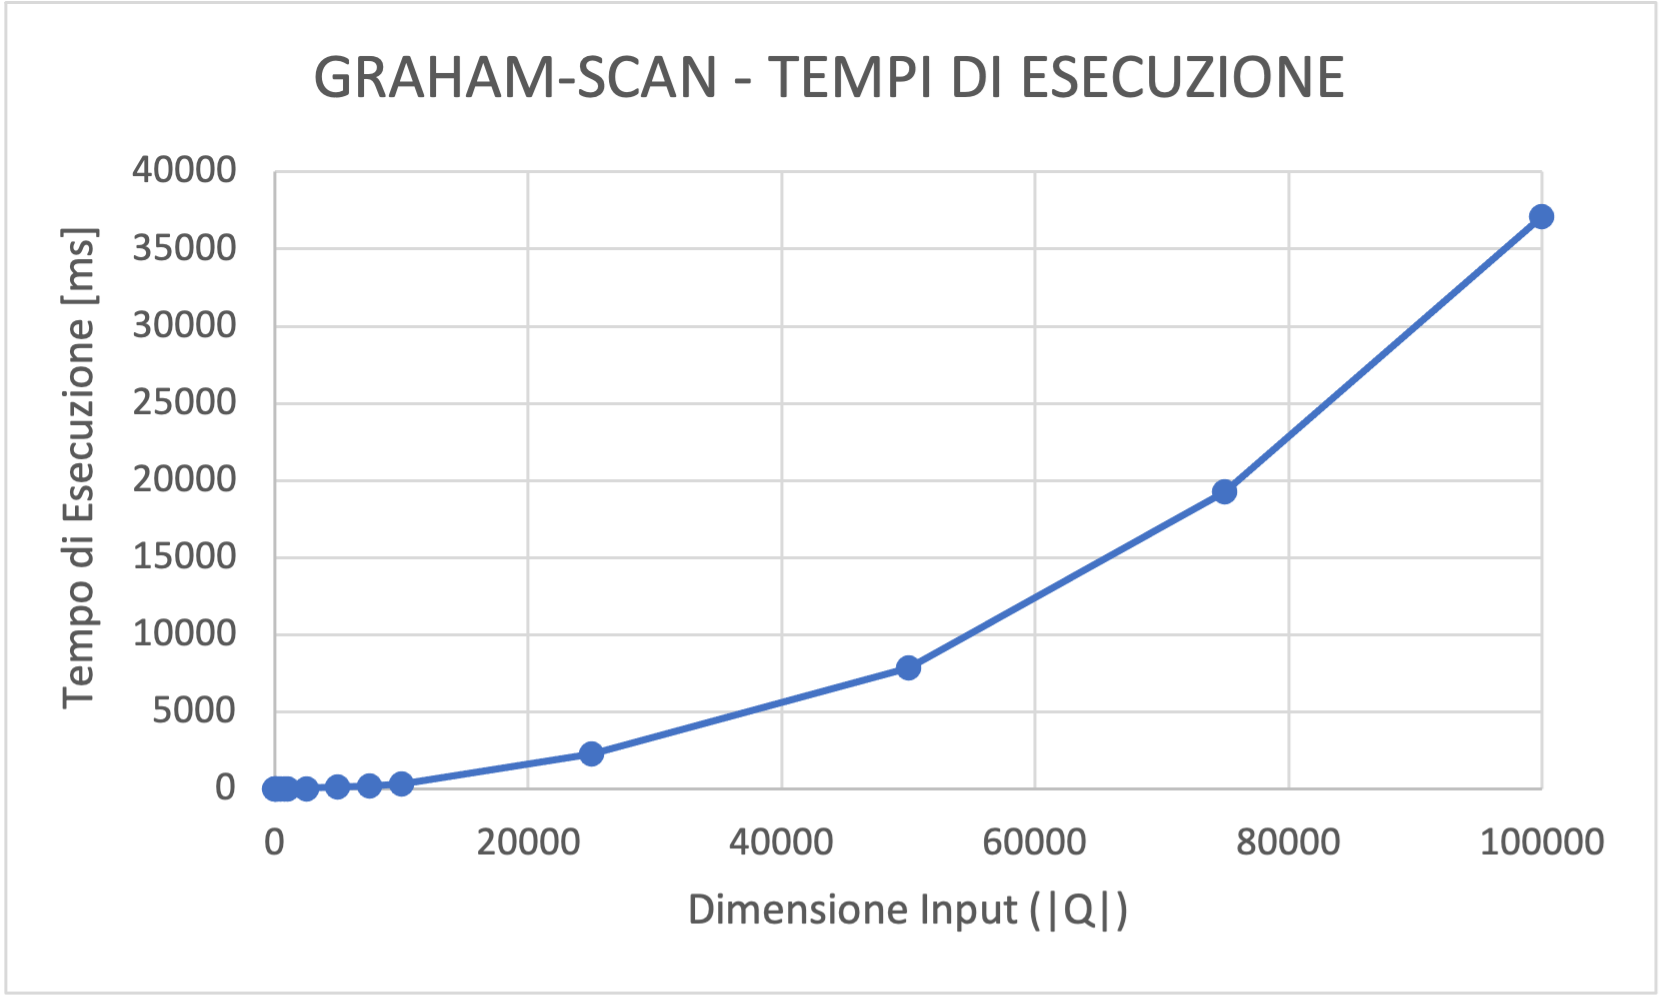
\includegraphics[width=0.8\linewidth]{datisperimentali.png}
    \caption{Tempi di esecuzione di \texttt{GRAHAM-SCAN(Q)}, al variare di $|Q|$.}
    \label{fig:graficodati}
\end{figure}

\pagebreak

\subsection*{\small{INTERFACCIA GRAFICA}}
Ino ltre, per visualizzare graficamente l'algoritmo, è stata implementata la classe \texttt{Test.java}, contenuta nella repository GitHub indicata alla fine dell'elaborato.\\

Come spiegato dettagliatamente nel file \texttt{README.md}, l'esecuzione di questa classe genera un insieme di 50 punti disposti in modo casuale nel piano e li mostra all'utente in una GUI. Quando l'utente preme il tasto "ENTER", la classe calcola l'involucro convesso dei punti generati (sfruttando la classe \texttt{GrahamConvexHull.java}) e lo mostra graficamente all'utente, come mostrato in Figura \ref{fig:GUIClass}.

\begin{figure}[ht]
    \centering
    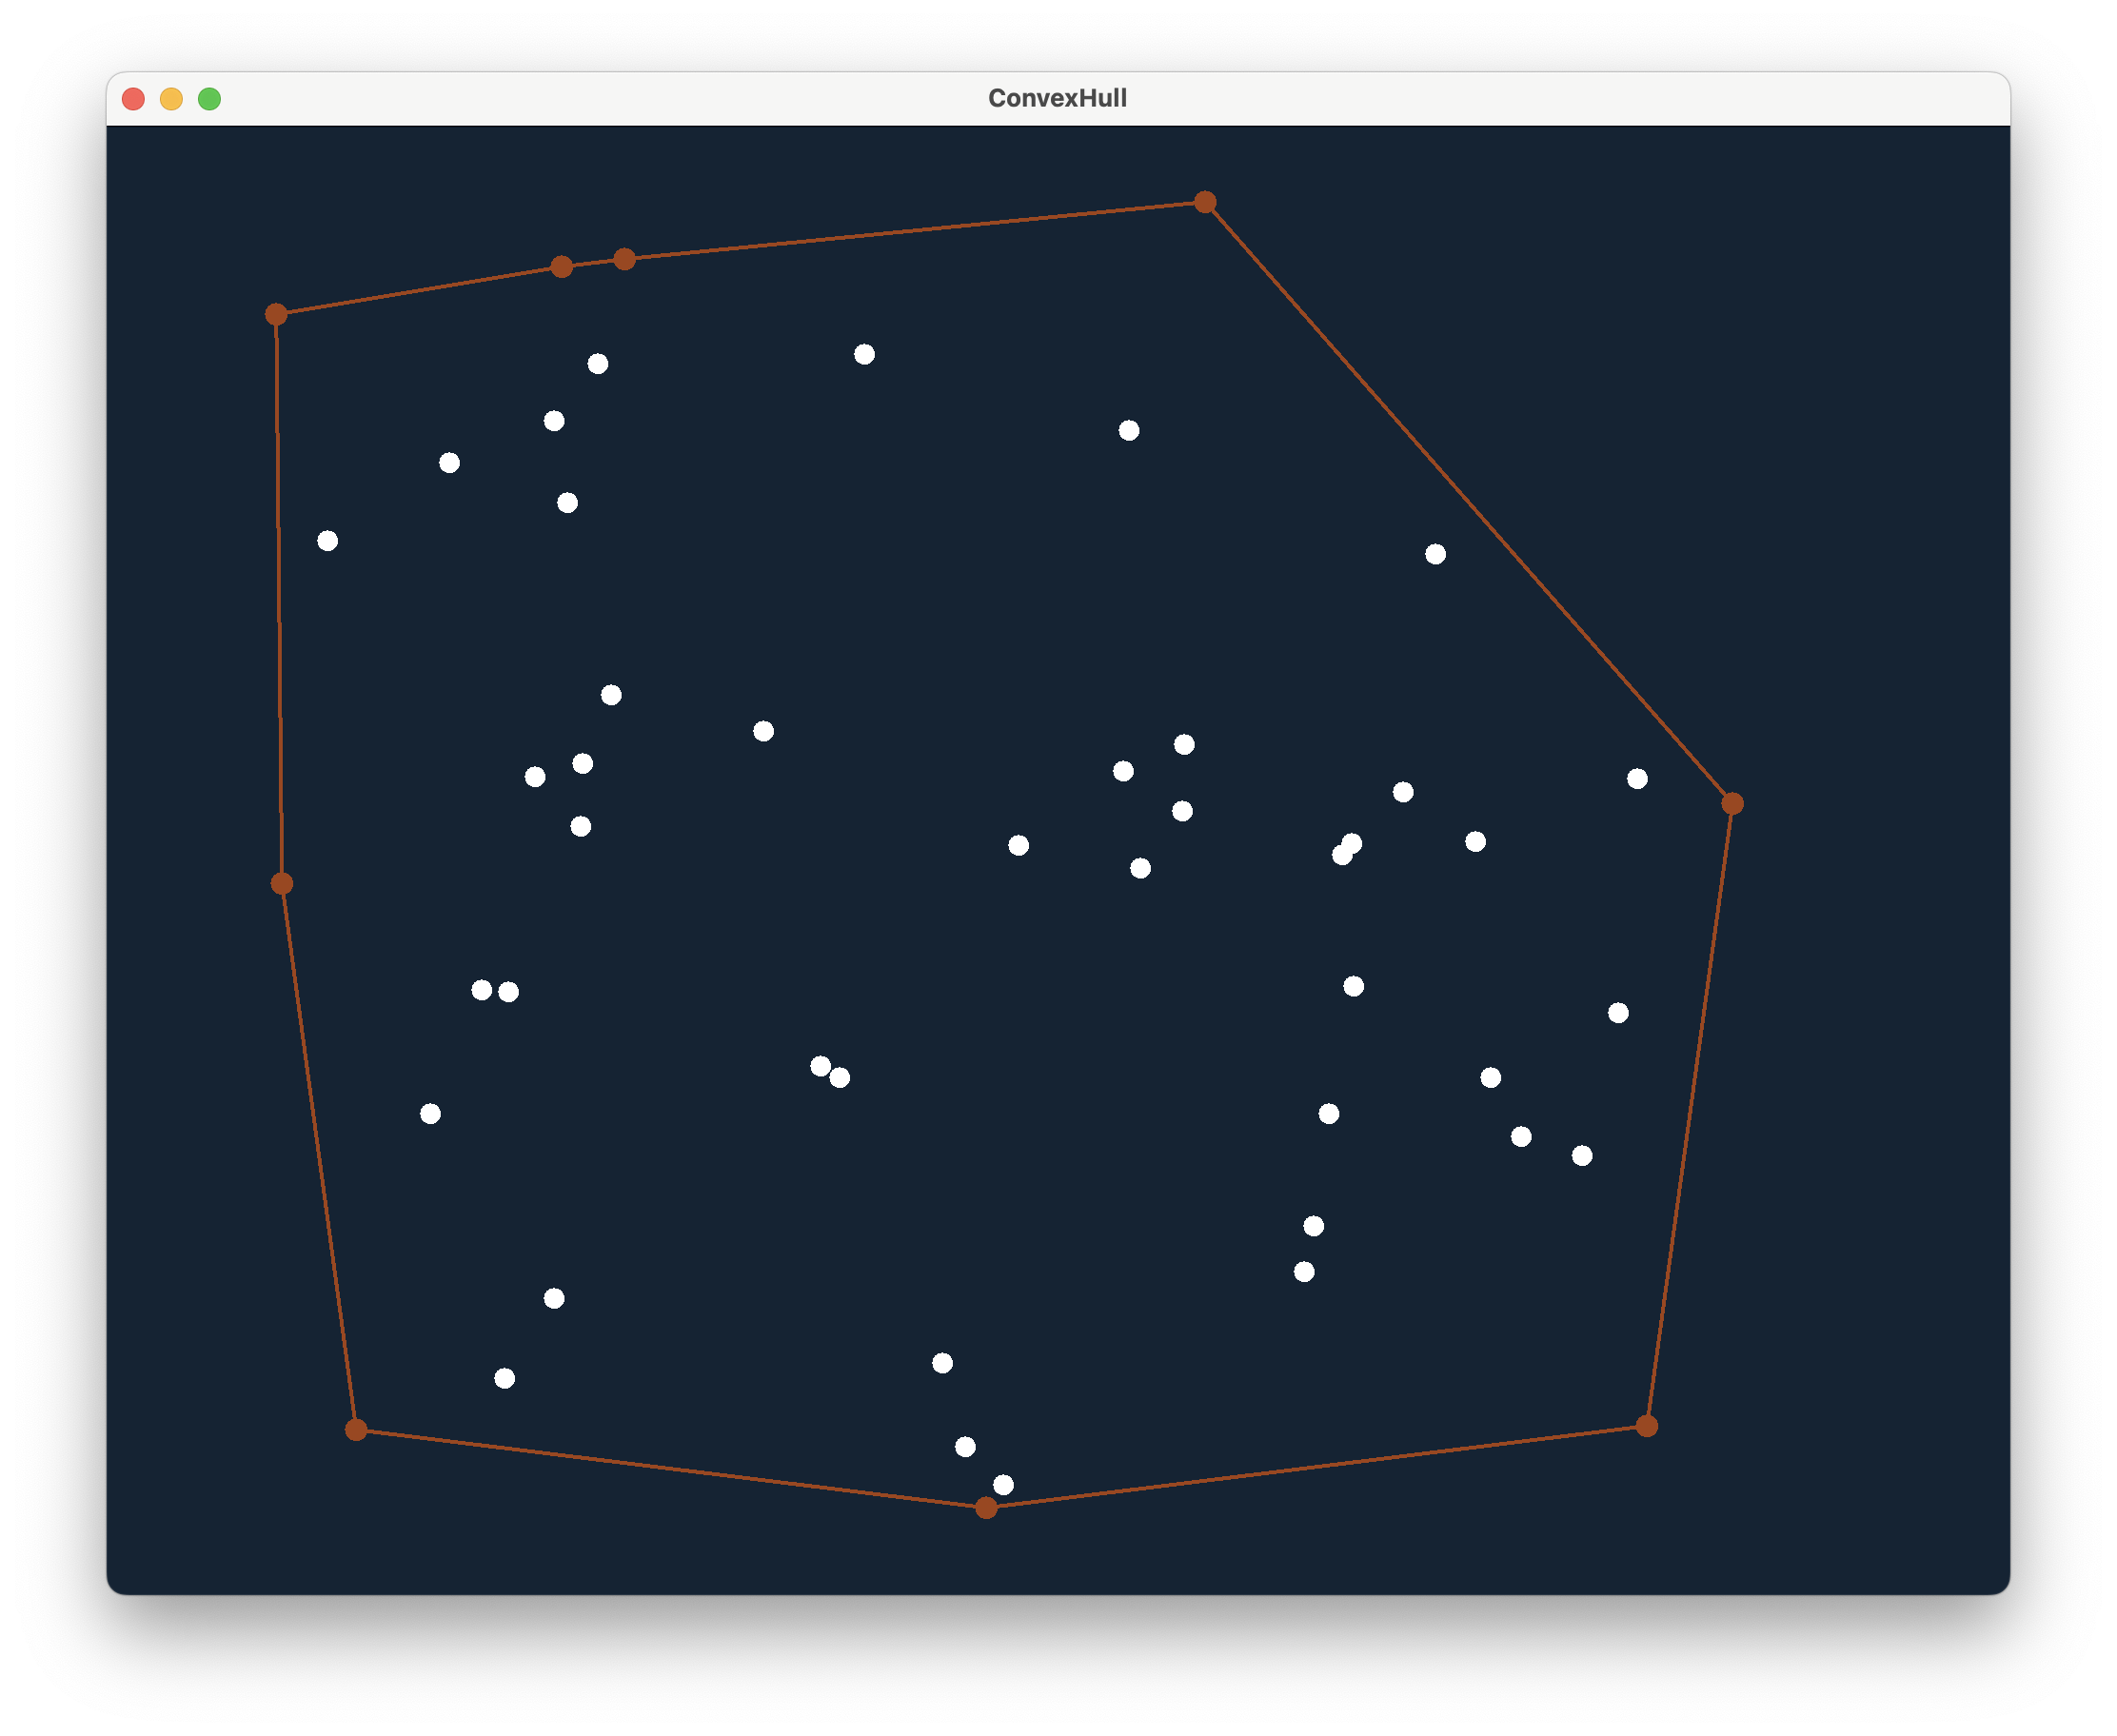
\includegraphics[width=0.75\linewidth]{GUIClass.png}
    \caption{Esempio di esecuzione della classe \texttt{Test.java}.}
    \label{fig:GUIClass}
\end{figure}

\chapter{Conclusioni}\label{ch:conclusioni}
In conclusione, in generale il problema del calcolo dell'involucro convesso di un insieme di punti $Q$, con $|Q| = n$, può essere risolto in un tempo $O(nlgn)$. L'unico algoritmo che migliora questa soglia è quello di Jarvis, ma solo a fronte di alcune configurazioni di input (che producano un numero di vertici dell'involucro $O(lgn)$).\\

Inoltre, l'algoritmo di Graham proposto risulta essere molto più facile da implementare rispetto ad altri metodi esposti (divide et impera, prune and search), che richiedono comunque lo stesso tempo di esecuzione. Questo perché Graham sfrutta semplicemente la definizione di prodotto vettoriale e la possibilità di ordinare un array di punti secondo l'angolo polare (sfruttando il prodotto vettoriale definito). Questo è semplicemente realizzabile dato che la maggior parte dei linguaggi di programmazione consente di ordinare elementi in un array (in particolare, in una lista) specificando la relazione di confronto tra due elementi (in questo caso l'angolo polare, discriminabile tramite prodotto vettoriale). Poi, le strutture dati necessarie sono elementari e quindi già implementate nei linguaggi di programmazione (a parte la funzione \texttt{NEXT-TO-TOP()}, la cui definzione è banale avendo \texttt{TOP()} a disposizione).

\pagebreak

% BIB
\nocite{*}
\bibliographystyle{unsrturl}
\bibliography{refs}

\vspace{10mm}

La repository pubblica contenente il codice dell'algoritmo di Graham sviluppato e alcune classi di prova è disponibile su GitHub:

\url{https://github.com/versi379/ConvexHull}.

\end{document}
% END DOCUMENT
